\cleardoublepage

\section{绪论}

\subsection{研究的背景与意义}

\par 随着近年来人们生活水平和医疗技术的不断提高,人类在面对疾病时也有了越来越多的手段以解决越来越多的疑难杂症,全球人类的平均寿命也在不断延长,然而,许多常见的癌症却不在此列。宫颈癌在女性常见的癌症中发病率高居第四位,严重威胁着女性的生命和健康。2018年,全球估计有57万女性被诊断出患有宫颈癌,约31.1万女性死于该疾病。然而,宫颈癌的发病过程是缓慢增长的,从癌前病变到病发的时间通常是5年或更长,这为通过早期科学有效的检测手段发现和适当治疗降低宫颈癌的发病率和死亡率提供了机会。全世界大约七成的宫颈癌发生在发展中国家\cite{wild2014world},在发达国家中,因为宫颈抹片筛查以及其他检测方法的普及,宫颈癌的发病率和致死率大大降低\cite{canavan2000cervical}。这也说明,定期进行科学的宫颈癌筛查是十分必要的。
\par 宫颈癌筛查主要由“细胞学-阴道镜-组织学”三阶梯诊断程序组成,其中,作为第一道检测手段的细胞学筛查的主要作用是通过较低的成本和较快的检测速度实现大量的、普遍的筛查,一般来说,医生会先通过细胞学检测手段对患者进行诊断,如果没有发现异常的病变情况,患者就不再需要进行后续的检测了。因此,细胞学检测手段除了应当注重检测成本与检测速度以外,还应提高对病变细胞或组织的敏感程度,应当尽量能够检测出所有的病变情况。而由于细胞学检测只是第一道检测手段,阴道镜与组织学的检测手段可以更轻易地取得更为精确的检测结果,由此,细胞学检查中对检测结果的准确性要求相对会低一点。
\par 在临床上,细胞学检查的主要手段就是TCT检查,即采用液基薄层细胞检测系统检测宫颈细胞并进行细胞学分类诊断。TCT检查通常需要医生使用专门的宫颈刷来采集子宫颈的脱落细胞样本,再将细胞样本漂洗后转移到保存液瓶中,然后放入全自动细胞检测仪中将细胞混匀、过滤、转移,并最后将细胞帖附到玻片上。之后需要将玻片进行染色固定才能在显微镜下通过估计细胞的类型和形态特征,如细胞核大小、核胞浆比进行观察诊断,最后按照Bethesda系统(TBS)的描述性诊断方法给出诊断报告。
\par 宫颈TCT筛查通常需要医生通过显微镜在整个玻片上、上亿个细胞中寻找病变或疑似病变的细胞,最后根据全片中病变细胞的状况给出诊断。通常情况下,整个TCT样本的片子含有几亿甚至几十亿像素,十分巨大;玻片上也有上亿细胞,数目非常多。可想而知,全人工的阅片过程十分耗时费力,需要非常大的工作量。但是,由于前文中我们提到的细胞学检测结果更关注对病变细胞的敏感程度,对病变检测准确性的要求相对较低的特点,我们可以通过深度学习的技术利用计算机辅助医生完成阅片的过程。
\par 我们可以设计一个对病变细胞较为敏感的系统,它可以自动地识别通过显微镜得到的TCT样本的扫描图片上几乎所有的病变细胞,然后医生就可以通过仅查看计算机给出的病变区域或潜在病变区域的病变情况给出相应的诊断,而不在需要在整个TCT样片中寻找病变区域。此外,我们甚至可以设计一个足够好的宫颈病变细胞检测系统,它除了对病变细胞有着足够的敏感性以外,还有着足够的准确性,这样,这一系统就可以在临床上自动地给出TCT检查的结果并报告病变细胞在TCT图片中的位置,完全在TCT阅片这一过程中将医生解放出来。
\par 除去帮助医生自动完成TCT阅片以外,通过计算机辅助阅片的方式还可以进一步改善TCT检查结果的准确性。这是由于医生在临床实践中,往往会在阅片的过程中遇到很多问题。

\begin{enumerate}
    \item TCT样本中细胞数目众多,可能会造成遗漏
          \par 如\ref{TCT全片}所示,一个TCT样本的片子通常含有上亿细胞,数目非常多。医生几乎不可能逐一检阅每个细胞,因此,在临床实践中医生在阅片的过程中可能会遗漏掉某些病变细胞,从而影响诊断结果的准确性。例如,在制片的过程中,如果部分病变等级较高的细胞恰好集中在了玻片的某一区域,而医生在阅片时恰好遗漏了这一区域,那么医生对TCT涂片的病变情况判断结果可能会更加偏向较低的病变等级,这就会导致诊断结果更倾向于较低的病变等级,这显然不利于医生做出准确的诊断结果,也不利于医生和患者获悉正确的病情。而且,这一过程使得诊断结果具有了一定的随机性,极度依赖于制片过程的混匀操作以及制片时病变细胞分布的均匀性,这就导致TCT检测结果可能在一定程度上不能准确描述患者的病情。

          \begin{figure}[h]
              \centering
              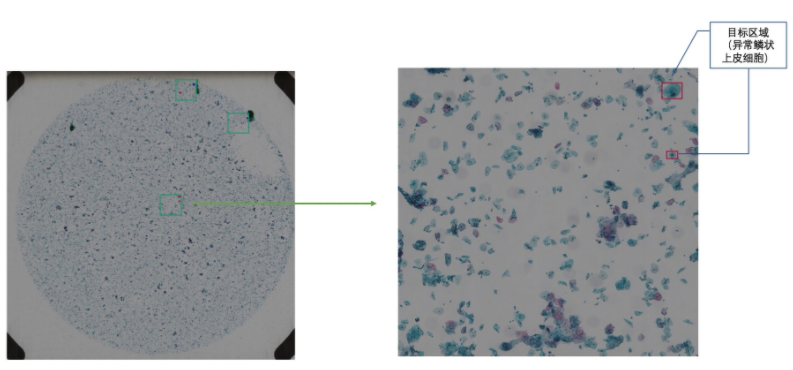
\includegraphics[width=0.5\paperwidth]{TCT/whole_pic.png}
              \caption{全片与部分视野的大小对比。左图为全片,右图为一个视野,在视野中可以看到正常细胞与病变细胞}
              \label{TCT全片}
          \end{figure}
    \item 类别判定的主观性
    \label{par:类别判定的主观性}
          \par 此外,全人工的阅片可能会导致诊断结果带有一定的主观性。某些类别的判定并没有十分明确的标准,这就导致医生在诊断时诊断结果可能会取决于医生的主观偏好。以\ref{HSIL-SQCA特征}为例,可以看到右图中部分被标注为HSIL的病变区域有着与SQCA区域几乎相同的形态特征而与左图中的HSIL类别的形态差异较大。这是因为在临床实践中,对于SQCA类别的检出,组织学的检查手段——组织病理切片相较于细胞学的检测手段——TCT检查有着高得多的准确性,而作为第一道检测手段的TCT检查,只要检测出较高的病变等级,那么患者就需要通过进一步的阴道镜、组织学等检测手段进行进一步的检查。换言之,在细胞学的检测手段中如果不论检测出HSIL还是SQCA,都需要患者进行进一步的组织学检查进行进一步的确定,而如果TCT图片中的细胞只是勉强达到SQCA的标准,这时如果给出SQCA的检查结果就存在误诊的可能性,而且可能会给患者带来较大的心里负担,因此,医生对于某些勉强达到SQCA标准的病变细胞,就更愿意标注为HSIL而不是SQCA。

          \begin{figure}[h]
              \centering
              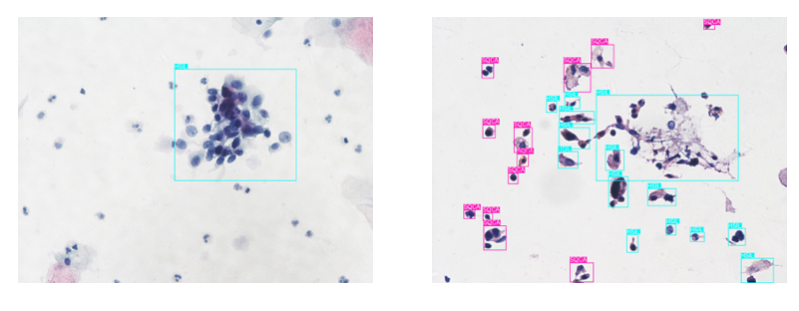
\includegraphics[width=0.5\paperwidth]{TCT/HSIL-SQCA.png}
              \caption{HSIL与SQCA两个类别的特征,左图为HSIL,右图为SQCA。全片与部分视野的大小对比。}
              \label{HSIL-SQCA特征}
          \end{figure}
\end{enumerate}
\par 由此,为了减少医生的工作量,避免诊断过程中因为人为原因造成遗漏等问题,并进一步提高诊断结果的准确性,我们亟需计算机的辅助诊断方法以实现快速、准确的宫颈癌筛查。

\subsection{论文主要研究内容}

\par 目前,利用计算机辅助医生完成TCT检查的阅片工作还存在许多难题。
\subsubsection{染色导致的色彩差异}
\par TCT检查所产生的图片中细胞的颜色并不是细胞本身的颜色,而是细胞被染色剂染色之后的颜色。因此,即使是同样的细胞部位、同样的病变程度,也可能因为染色剂的不同而呈现出不同的颜色状态。不仅如此,输入到计算机中的视野图片并不一定是TCT检查刚刚做完时的视野图片,而染色剂会随着时间慢慢褪色。不同染色剂品牌,不同颜色的染色剂都会有不同的褪色速率,因此,即使是同一份TCT涂片也可能因为输入计算机系统的时间不同而表现出不同的色彩状态。
\begin{figure}[h]
    \centering
    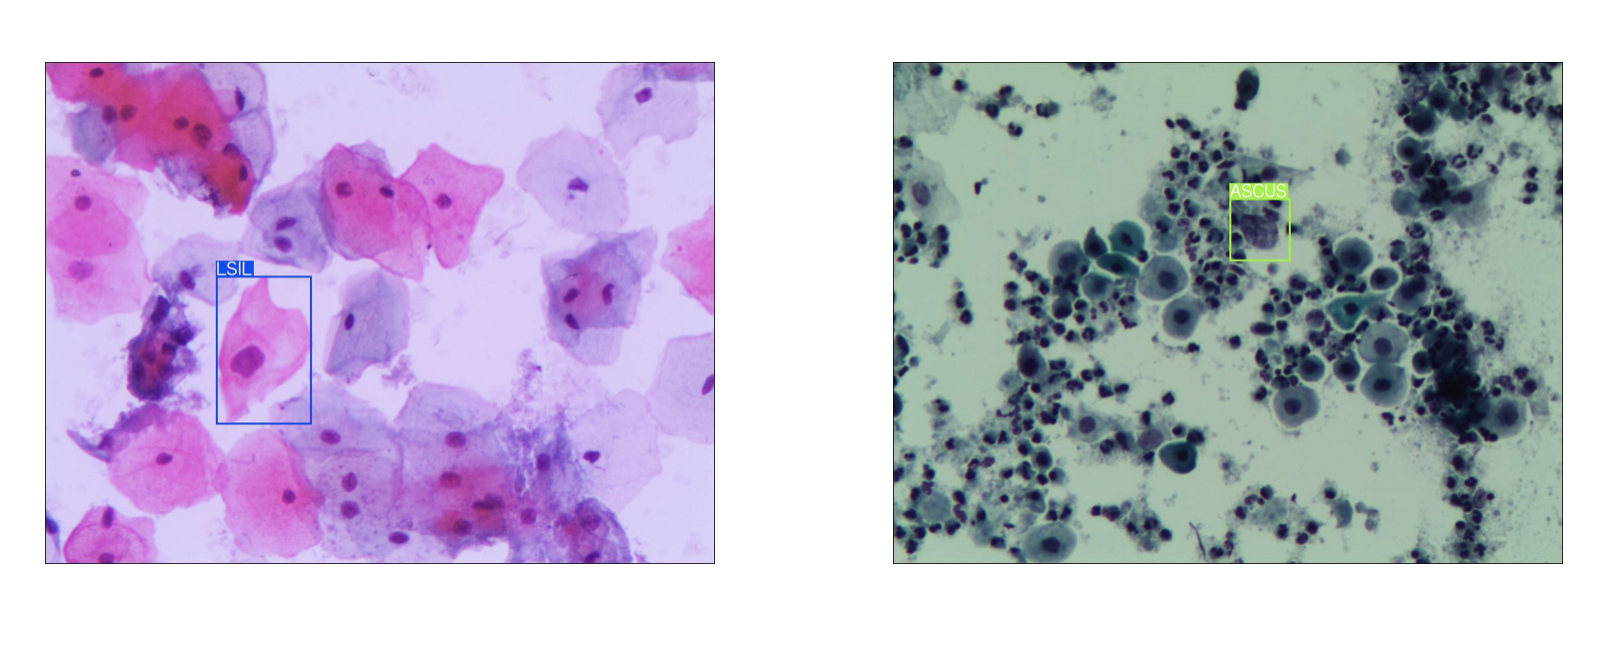
\includegraphics[width=0.5\paperwidth]{TCT/色彩差异.png}
    \caption{不同样片之间由于使用的染色剂不同、褪色时间不同等原因表现出完全不同的色彩特征}
    \label{论文色彩差异}
\end{figure}
\subsubsection{单细胞与细胞簇的形态差异}
\label{par:单细胞与细胞簇的形态差异}
\par 医生在标注病变细胞框的时候,如果病变细胞是单个存在的、周围没有其他细胞的状态,那么医生会给该细胞单独标注一个框。但是,如果病变细胞聚集在一起形成了一个很大的细胞簇,那么病变细胞之间的界限会变得十分糢糊,只能选择标注一个很大的框将整个细胞簇框住。这就导致了同一种类标签的标注框有着两种不同的含义——既可以是单个的病变细胞,也可以是一整个病变细胞簇,而二者在形态上有着巨大的差异。
\par 例如,由于不论是病变细胞还是正常细胞细胞核往往在形态上处在整个细胞中心的位置,那么单个细胞对应的框的中心一般来说就是这个细胞的细胞核,因此从该处往往可以获得细胞核的形态特征。换句话说,如果网络发现了细胞核的形态特征,就可以将该点作为检测框的中心的进行预测。但是,如果框中的是一个大的细胞簇那么其中心就不再是明显的细胞核的特征了。而细胞核的形态特征又是判断病变与否已经病变种类的相当关键的特征,这就导致网络的学习过程中可能遇到难以学习的特征形态。与此类似的,单个细胞框的周围会是细胞质边界的特征,这也是判断病变细胞的一个重要特征,但是细胞簇的边缘是多个细胞聚集在一起时组成的形状,因为细胞是经过混匀的,这一形态信息完全由混匀过程决定可以认为是随机的,这对判断细胞的病变程度毫无意义。
\par 此外,单个细胞与细胞簇的界限并没有那么明显。例如,医生在标注框的时候,会遇到两三个细胞挨在一起的情况,这种情况下可以说为每个细胞单独标注框和将这两三个细胞视作一个细胞簇只标注一个框都是合理的。但这就给网络的学习带来了很大的难度——网络不仅要学会如何判断病变细胞,还需要学会制作训练用数据集的医生对于上述情况的偏好情况。而事实上,由于数据的标注由不止一位医生完成,往往每位医生对都上述情况会有不同的偏好,因此,网络可能根本无法学习到这一规律。这一问题严重地阻碍了网络的学习过程,然而,在实践中,我们往往并不关注病变细胞是有单独的框还是由一个框标注出来的,我们更关心病变细胞的召回率和病变等级判定的准确率。
\begin{figure}[h]
    \centering
    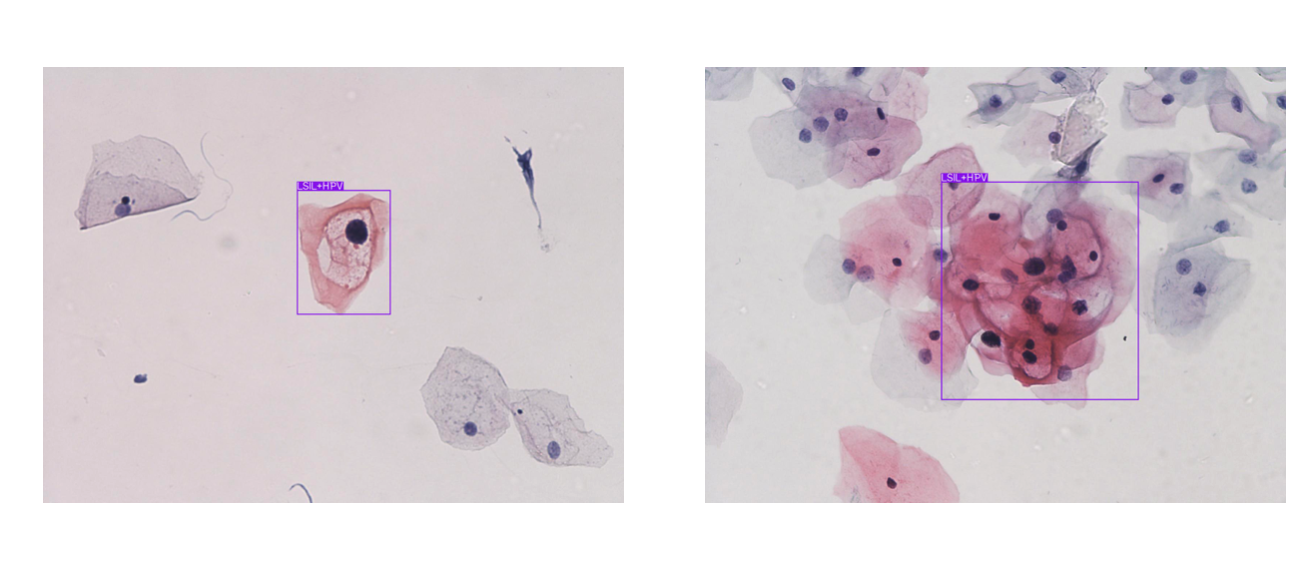
\includegraphics[width=0.5\paperwidth]{TCT/single_multi.png}
    \caption{单个病变细胞与病变细胞簇形态差异比较,左图为单个病变细胞,右图为许多病变细胞形成的细胞簇,两图中的病变细胞均为统一病变等级,但是由于细胞数目不同而具有完全不同的形态特征}
    \label{论文形态差异}
\end{figure}
\subsubsection{放大倍率不一致}
\par TCT检查的图片都是经过显微镜放大的,所以图片中细胞的绝对大小并没有实际的意义,甚至这一大小的变换还会为网络的学习带来阻碍。例如,涂片中可能出现一种叫做炎细胞的正常细胞,它相比入一般细胞会小得多,医生在做诊断时可以自然地忽略它,但是它的形态特征在放大之后与最高等级的病变细胞——鳞癌细胞的形态特征十分相近。他们的区别只是炎细胞相较与正常细胞非常小,而鳞癌细胞具有正常细胞的大小尺度。现有的深度学习方法主要通过FPN来生成各种尺度的图像金字塔来处理这种尺度变换的问题,但是,这种方法更适合用来检测尺度大小不确定的目标,对于形态特征相近只有尺度不同的目标,这种方式反而会影响网络的训练。
\begin{figure}[h]
    \centering
    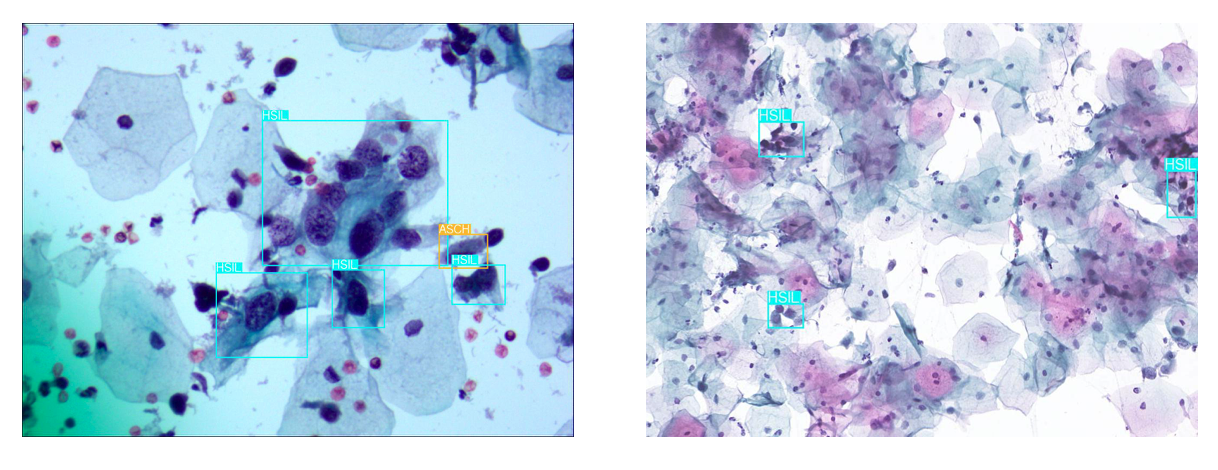
\includegraphics[width=0.5\paperwidth]{TCT/scale.png}
    \caption{不同图片之间放大倍率有着较大的差距,左图中的正常细胞大小相较右图中大得多,而实际上正常细胞的大小应当是一致的,所以左图放大倍率应当比右图高很多}
    \label{论文倍率差异}
\end{figure}
\par 在本文中,我们主要关注单细胞与细胞簇的形态差异与图片放大倍率不一致这两个问题。
